\documentclass[11pt,a4paper]{book}

\usepackage{Appunti}

\begin{document}
\title{Clean Code\\
\large{\textit{Robert C. Martin}}}
\author{Jacopo De Angelis}
\maketitle

\pagebreak
\tableofcontents
\pagebreak

\chapter{Clean code}
Il codice non finirà con l'era dell'autogenerazione da IA. Qualcuno dovrà creare le IA, qualcuno dovrà imparare come dare le specifiche. Il codice sarà sempre presente.

\section{Pessimo codice}
Una delle prime cause del pessimo codice è la fretta dettata dall'ansia. L'idea di dover far uscire il codice il prima possibile ci porta a commettere errori, commettere inesattezze. Quello è ciò che può portare a seri problemi successivamente, il rileggere il proprio codice scritto in maniere quantomeno esecrabili è una tortura. E ricordiamo che se si pensa "lo metto a posto dopo", dopo equivale a mai.

I rallentamenti derivanti da nuovo codice di bassa qualità sono esponenziali, lentamente la produttività crolla perchè operare sul codice precedente è sempre più complicato.
\begin{figure}[h!]
	\begin{center}
		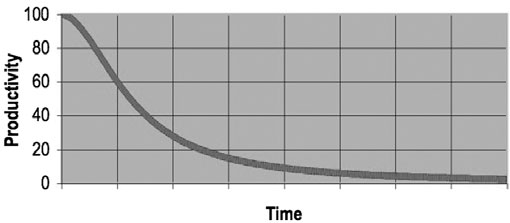
\includegraphics[scale=0.6]{img/001.png}
		\caption{Produttività vs tempo}
		\label{fig: 001}
	\end{center}
\end{figure}

Il che può portare ad un desiderio di ricreare da zero l'intera base del codice, cosa non solo dispendiosa ma che richiede anche molto tempo. I team si trovano a lavorare in parallelo, il nuovo team che ricrea tutto e integra il nuovo lavoro del vecchio team e, alla fine, ci si troverà nella stessa situazione.

\section{Scrivere buon codice}
Scrivere buon codice richiede disciplina nell'uso di molte piccole tecniche applicate in ogni singolo momento. Tutto questo richiede anche una parte di "senso estetico", un percepire il perchè un bel codice sia, appunto, bello.

Una regola che possiamo ereditare dai boy scout: lascia il campo più pulito di come l'hai trovato. Ad esempio: una variabile può avere un nome più autoesplicativo? Cambiala. Una funzione può essere spezzata in più funzioni elementari? Dividila.

\chapter{Nomi significativi}
\section{Usare nomi che rivelino l'intenzione}
Trovare nomi significativi non è semplice ma il tempo che prendono nel farlo è sicuramente meno di quello speso a decifrare nomi non chiari.

Ogni nome, che sia di variabile o di funzione, deve rispondere alle domande:
\begin{itemize}
	\item[] Cosa fa
	\item[] Perchè esiste
	\item[] Come viene utilizzata
\end{itemize}
Se un nome richiede un commento allora il nome è sbagliato.

Ad esempio
\lstinputlisting[language=]{code/001}\label{code: 001}
d non dice molto come nome. Dovremmo scegliere un nome migliore, ad esempio
\lstinputlisting[language=]{code/002}\label{code: 002}
Scegliere un nome che rivela un intento rende molto più semplice cambiare e comprendere un codice. Ad esempio cosa fa questo pezzo di codice?
\lstinputlisting[language=]{code/003}\label{code: 003}
Il problema di questo codice non è la sua semplicità ma la sua capacità di avere un senso implicito. Ad esempio, le domande che ci possiamo porre sono:
\begin{itemize}
	\item[] Cos'è theList?
	\item[] Che significato ha l'elemento 0 di theList?
	\item[] Qual è il significato di 4?
	\item[] Come viene usata la lista ritornata?
\end{itemize}

Queste risposte dovrebbero essere nel codice. Immaginiamo ora di lavorare a campo minato. Rinominiamo la lista con gameBoard.

Ogni cella della board è rappresentata da un array, il valore alla posizione 0 è la posizione dello status della cella e se è 4 vuol dire "segnata". Già dando implicitamente queste notazioni possiamo migliorare il codice:
\lstinputlisting[language=]{code/004}\label{code: 004}

Possiamo andare anche oltre e scrivere una semplice classe per le celle invece di avere degli int. Può includere una funzione con un nome che ne sveli l'intento per nascondere questo numero. Il risultato è:
\lstinputlisting[language=]{code/005}\label{code: 005}

\section{Evitare la disinformazione}
Mai usare parole che non descrivono la realtà, ad esempio usare accountList solo se effettivamente ci troviamo davanti ad una List.

Non usare nomi che variano tra di loro per dei piccoli dettagli, ad esempio \emph{XYZControllerForEfficient\textbf{Handling}OfStrings} e \emph{XYZControllerForEfficient\textbf{Storage}OfStrings}

Avere una naming convention consistente è essenziale. Un pessimo esempio di uso è quello di o ed l minuscoli, pericolosamente simili a 0 e 1.

\section{Fare distinzioni significative}
Evitare nomi con degli errori di battitura intenzionali perchè si vogliono nominare due variabili allo stesso modo. Evitare anche nomi che non danno informazioni, ad esempio:
\lstinputlisting[language=]{code/006}\label{code: 006}

Evitare nomi "che creano rumore", ad esempio ProductInfo e ProductData si differenziano per la seconda parola ma comunque non sappiamo cosa facciano.

Il tipo di entità non dovrebbe mai essere contenuto nel nome. NameString non ha senso, non ci chiederemmo mai se un semplice Name possa essere un float, questo perchè il nome stesso ci informa del suo contenuto.

Un esempio di confusione è:
\lstinputlisting[language=]{code/007}\label{code: 007}
Come potremmo mai sapere quale funzione chiamare dal suo nome?

Distinguere sempre i nomi in modo da intuire immediatamente la loro funzione leggendoli.

\section{Usare nomi pronunciabili}
Devi poterlo pronunciare. Hai mai provato a discutere della funzione della classe Genymdhms (generation date, year, month, day, hour, minute, and second)? Spero di no.

Immaginiamo comparare questa classe
\lstinputlisting[language=]{code/008}\label{code: 008}
con questa
\lstinputlisting[language=]{code/009}\label{code: 009}

\section{Usare nomi ricercabili}
Le variabili con nome di una singola lettera vanno bene solo come variabili locali di un metodo, mai in altro modo, sarebbe impossibile cercarle altrimenti.

Compariamo
\lstinputlisting[language=]{code/010}\label{code: 010}
con
\lstinputlisting[language=]{code/011}\label{code: 011}

\section{Prefissi}
I prefissi erano utili anni fa, ormai sono abbastanza inutili.

\section{Interfacce e implementazione}
Ci sono due scuole di pensiero:
\begin{enumerate}
	\item Interfaccia che inizia con I, implementazione senza decorazioni (IClasse, Classe)
	\item Interfaccia senza decorazioni, implementazione con suffisso Imp (Classe, ClasseImp)
\end{enumerate}

É uguale.

\section{Evitare il mapping mentale}
Il significato dei nomi non deve essere chiaro solo a chi scrive ma anche a chi legge.

\section{Nomi delle classi}
Le classi dovrebbero essere nomi o frasi di sostantivi, evitare Manager, Processor, Data o Info. Una classe non dovrebbe essere un verbo

\section{Nomi dei metodi}
I nomi dovrebbero contenere un verbo che descrivere cosa fanno, ad esempio postPayment, deletePage o save.

Accessori, mutatori e predicati dovrebbero iniziare con get, set e is.

\section{Non usare nomignoli}
Non chiamare variabili, metodi e classi con nomi che utilizzano inside joke, riferimenti culturali o battute. Chiamare la funzione delete() holyHandGranade non è simpatico, è un inferno.

\section{Una parola per concetto}
Scegli una parola che esprima un concetto e mantienila. Ad esempio scegli tra fetch, retrieve e get e poi usa solo quella, non alternare tra le tre.

\section{Usare nomi del dominio della soluzione}
Meglio usare nomi che hanno un significato speciale nel caso sia quello il caso. Ad esempio, dire AccountVisitor vuol dire molto se si è a conoscenza del pattern visitor. I nomi che usano un lessico tecnico sono comodi.

\section{Usare nomi del dominio del problema}
Nel caso non ci siano nomi immediati da utilizzare facenti parte del dominio della soluzione, allora possiamo iniziare a guardare il dominio del problema.

\section{Aggiungere un contesto significativo}
Solitamente è meglio avere nomi che si spieghino da soli, in certi casi, però, ciò è difficile. Prendiamo ad esempio firstName, lastName, street, houseNumber, city, state e zipcode. Assieme sappiamo che sono un indirizzo ma presi singolarmente? Se vedessimo state usato da un'altra parte? In questo caso, allora, può essere accettabile usare, ad esempio addrFirstName, addrLastName, addrStreet, addrHouseNumber, addrCity, addrState e addrZipcode.

Non bisogna aggiungere del contesto a caso però, ad esempio dando a tutte le variabili un prefisso che descriva l'app.

\chapter{Funzioni}
La maggior parte delle regole di scrittura per le funzioni sono le stesse descritte dalle buone norme del \href{https://refactoring.guru/refactoring/techniques}{refactoring}.

\section{Corte}
Le funzioni dovrebbero essere lunghe massimo intorno alle 20 righe, nulla vieta di riuscire a ridurle ulteriormente però. Se è di più possiamo chiederci "è possibile estrarre una parte della funzione"?

Ad esempio la funzione
\lstinputlisting[language=]{code/012}\label{code: 012}
è riscrivibile come
\lstinputlisting[language=]{code/013}\label{code: 013}

\subsection{Blocchi e indentazione}
Se possibile sarebbe meglio ridurre i blocchi di indentazione a una sola linea, come abbiamo visto nel codice precedente, e possibilmente che chiami un'altra funzione per svolgere le sue funzioni.

Tutto ciò rende il codice snello e leggibile

\section{Fare una sola cosa}
Un metodo non deve fare tutto e male ma solo una cosa e farla bene. Un metodo che si occupa di una sequenza di passi avrà richiami a metodi che eseguono le subroutine ma non avrà altra logica al suo interno.

Se in una funzione vediamo più sezioni come dichiarazione, inizializzazione e scrematura come possiamo vedere qua
\lstinputlisting[language=]{code/014}\label{code: 014}
vuol dire che probabilmente possiamo scomporla ulteriormente.

\section{Un livello di astrazione per funzione}
Ci si deve assicurare che una funzione sia ad un solo livello di astrazione. Non dovremmo mai avere funzioni ad alto livello di astrazione mischiate a codice a basso livello di astrazione, crea solo confusione e non rispetta il principio di responsabilità.

\subsection{Leggere il codice dall'alto verso il basso}
Primo avviso: questo si applica solo a linguaggi compilati e a linguaggi che si occupano dell'analisi di tutto il codice prima dell'esecuzione. In un linguaggio interpretato questa regola non si applica in quanto le funzioni devono essere descritte bottom-top.

Come regola di base dovremmo poter leggere il codice come una narrativa, dalla funzione principale a quelle ausiliarie, scendendo sempre più tra i vari livelli di astrazione.

\section{Controlli di flusso}
É difficile mantenere brevi gli switch e gli if/else. Possiamo però separare lo switch in una classe di basso livello e non vederlo mai ripetuto.

Consideriamo questo codice
\lstinputlisting[language=]{code/015}\label{code: 015}
\begin{enumerate}
	\item è già grande e crescerà ancora di più all'aumentare delle tipologie di dipendenti
	\item fa più d una cosa
	\item viola il principio di singola responsabilità
	\item viola il principio open close\footnote{Le entità dovrebbero essere aperte per l'estensione, chiuse per le modifiche} perchè deve essere cambiata per ogni modifica nel dataset
\end{enumerate}

La soluzione a questo problema, ad esempio, è una \href{https://refactoring.guru/design-patterns/abstract-factory}{abstract factory}. La factory passerà l'istanza dei dipendenti e i vari metodi sono creati polimorficamente usando le interfacce.

Una regola possibile è che gli switch:
\begin{enumerate}
	\item devono compararire solo una volta
	\item devono sfruttare il polimorfismo
	\item devono essere nascosti tramite ereditarietà
\end{enumerate}
\lstinputlisting[language=]{code/016}\label{code: 016}

\section{Usare nomi descrittivi}
Così come per le variabili, i nomi devono essere significativi. Meglio un nome lungo rispetto ad un nome che non spiega ciò che accade nel metodo.

Importante è avere una naming convention, anche non scritta, in modo che i nomi siano consistenti e che siano facilmente interpretabili.

\section{Argomenti delle funzioni}
Il numero ideale di argomenti per le funzioni è 0. Uno va bene, due accettabile, tre già è strano, quattro o più richiede una giustificazione seria.

\subsection{Forma comune per singolo argomento}
Ci sono due ragioni per passare un argomento:
\begin{itemize}
	\item stai ponendo delle domande su di esso
	\item stai operando su di esso
\end{itemize}

Un altra ragione è quella di generazione di un evento: il metodo ha in ingresso un argomento ma in uscita nessuno.

\subsection{Argomenti di guardia}
Sono brutti. Passare un boolean in una funzione come guardia per dire con che modalità eseguire la funzione è brutto a vedersi. Sarebbe meglio dividere la funzione in più metodi.

\subsection{Funzioni con due argomenti}
Una diade non per forza è negativa, ad esempio quando si crea un punto è necessario passare due variabili per gli assi x e y e ciò è giusto. Il problema è quando ci troviamo davanti ad altre forme come, ad esempio, \emph{assertEquals(expected, actual)}. Quale viene prima, quale dopo? Serve pratica perchè non c'è un ordine naturale.

Le soluzioni sono svariate, ad esempio estrarre un campo e renderlo appartenente alla classe.

\subsection{Oggetti come argomenti}
Spesso se vengono passati due o tre argomenti, questi saranno legati in qualche modo, probabilmente in un oggetto. In quel caso è meglio pensare di passare l'oggetto direttamente. Ad esempio qua è visibile la differenza di lettura dei due metodi.
\lstinputlisting[language=]{code/017}\label{code: 017}

\subsection{Lista come argomento}
L'utilizzo delle liste opzionali di argomenti è molto comodo e in certi casi aiuta a tenere pulito il codice. Ad esempio
\lstinputlisting[language=]{code/018}\label{code: 018}
A tutti gli effetti ha due argomenti ma a runtime può essere usato con infiniti argomenti.

\subsection{Verbi e parole chiave}
Usare una combinazione di verbi per le funzioni e sostantivi per gli argomenti può rendere le funzioni molto evocative. Ad esempio \emph{writeField(name)} subito fa capire che questo nome verrà scritto.

Codificare le variabili nel nome del metodo è anche un metodo interessante per renderla autodescrittiva. Tornando all'\emph{assertEquals(expected, actual)} di prima, quando sarebbe più immediato e meno confusa la sequenza se si chiamasse \emph{assertExpectedEqualsActual(expected, actual)}?

\section{Non devono avere effetti collaterali}
Gli effetti collaterali sono bugie. Una funzione dovrebbe fare una e una sola cosa, nascondere un effetto collaterale, ovvero l'agire su di una variabile esterna al suo scope, è un modo di farle fare più cose.

Ad esempio:
\lstinputlisting[language=]{code/019}\label{code: 019}
Qua evidentemente inizializza la sessione quando la funzione dovrebbe solo validare l'utente. Questo va contro il principio di singola resposabilità

\section{Output}
Certi nomi possono confondere, portando a chiedersi se stiano parlando dell'input o dell'output. Ad esempio \emph{appendFooter(s)} attacca s ad un footer o attacca un qualche footer ad s? Solo guardando la firma del metodo si scopre che
\lstinputlisting[language=]{code/020}\label{code: 020}
effettivamente attacca un footer al buffer passato.

Quello che abbiamo appena fatto è un controllo secondario, un qualcosa che può interrompere il flusso di programmazione.

In generale gli output dovrebbero essere evitati, se possibile è meglio far agire le funzioni sull'oggetto che le possiede.

\section{Separazione dei comandi}
Una funzione dovrebbe fare qualcosa o rispondere a qualcosa, non entrambe.

\section{Preferire le eccezioni al ritornare direttamente messaggi di errore}
Passare errori direttamente porta al doverli gestire subito, invece passare un'eccezione ha due benefici principali:
\begin{itemize}
	\item sono rapidi da usare e non si confonde ciò che può essere passato
	\item possono essere messi in calce al percorso di esecuzione
\end{itemize}

\subsection{Estrarre i blocchi try/catch}
Con ciò si vuole dire di non scrivere l'interno del blocco catch con tutti i suoi passaggi ma di portarlo fuori come metodo in modo da avere una struttura molto più compatta, leggibile e gestibile. Ricordiamo che le eccezioni vanno gestite il più vicino possibile alla fonte ma non per questo non possiamo mandarle alla funzione chiamante.
\lstinputlisting[language=]{code/021}\label{code: 021}

\subsection{La gestione dell'errore è una sola cosa}
Le funzioni dovrebbero fare una sola cosa + la gestione dell'errore è una sola cosa = Una funzione che gestisce l'errore non dovrebbe fare altro. Ciò vuol dire che se in una funzione eiste la parola try dovrebbe essere la prima e niente dopo i blocchi catch e finally.

\subsection{Error.java e la dipendenza da esso}
Molti scrivono i messaggi di errore in una enumerazione da importare in ogni classe che la sfrutta. Risultato? Dipendenze ovunque ed essere costretti a modificare codice e ricompilare ogni volta.

Creare eccezioni figlie della classe Error invece rende il codice meno codipendente e più manutenibile.

\subsection{Non ripetersi}
Mai ripetere funzioni, piuttosto meglio importarle ma scrivere più volte lo stesso codice porta a dover debuggare più volte e c'è il rischio di riparare da una parte e non dalle altre.

\section{Programmazione strutturata}
Molti programmatori seguono il principio di Dijkstra: ogni funzione e ogni blocco deve avere una sola entrata e una sola uscita. Ciò vuol dire:
\begin{itemize}
	\item un solo return
	\item niente break o continue
	\item mai un goto
\end{itemize}

Questa regola perde di valore quando le funzioni sono molto brevi, questo perchè una sovraingegnerizzazione in un piccolo blocco di codice rischia di oscurare il vero significato dietro al metodo.

\section{Come si scrivono funzioni così?}
Ricorda: primo passaggio è la stesura, il successivo la pulizia. Va bene scrivere codice leggibile solo da te all'inizio, non devi lasciarlo così poi. Poco alla volta puoi pulirlo, renderlo perfetto.

\section{Esempio finale}
\lstinputlisting[language=java]{code/022}\label{code: 022}

\chapter{Commenti}
I commenti possono essere molto utili come anche superflui. Se imparassimo a scrivere codice comprensibile non ci servirebbe minimamente scrivere commenti. Spesso vengono inseriti per sopperire ad una mancanza del linguaggio.

Attenzione: commenti e documentazione non sono per niente la stessa cosa.

Tutto ciò vuol dire che nel momento nel quale si sente il bisogno di scrivere un commento bisogna chiedersi: posso scrivere il codice in modo che non serva?

Uno dei motivi principali di questa pratica è che il codice cambia, il commento spesso no.

I commenti non correggono del pessimo codice!

\section{Spiegati nel codice}


\end{document}